\section{Support Vector Machine (SVM)} \label{sec:prob2}
In this section, we consider the Support Vector Machine (SVM) for binary classification of several 2D datasets.

\subsection{Part 1}
First, we implemented the dual form of a linear SVM with slack variables.

[dual svm eqns]

I first converted the input data into a standard format, then we used the cvxopt Python package to execute the quadratic programming to find the desired $\alpha$ values.

[data format P, etc.]

With the simple 4 element dataset $\{((2,2),+1),((2,3),+1),((0,-1),-1),((-3,-2),-1)\}$, the algorithm outputs $(2,2)$ and $(0,-1)$ as the support vectors, meaning they lie on the boundaries of the margin, seen in~\cref{fig:2_1_decisions}.
The weight vector has elements $w = [0.308, 0.462]$ and bias, $b = -0.538$.
The training error is zero for this simple dataset.
We use regularization term $C=1$ for all results in this and the next subsection.

\begin{figure}
	\centering
	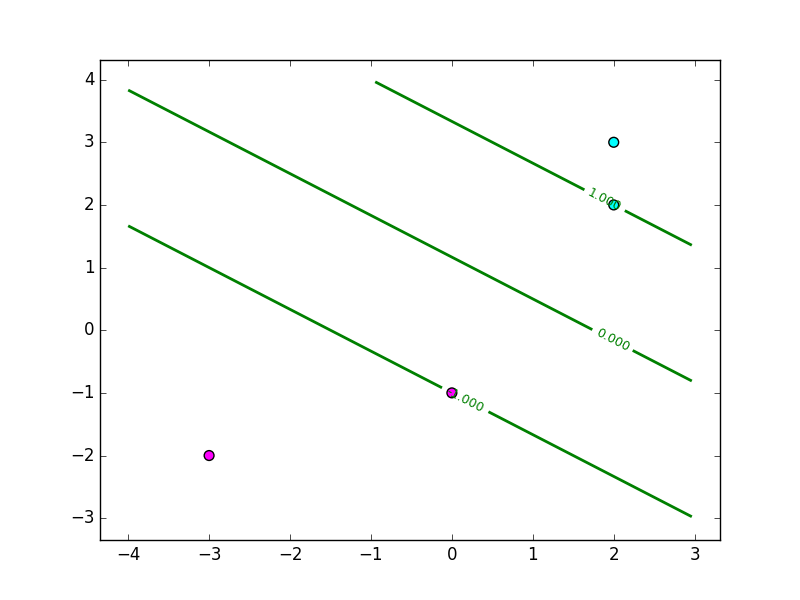
\includegraphics [trim=0 0 0 0, clip, angle=0, width=0.8\columnwidth,
	keepaspectratio]{figures/2_1_decisions}
	\caption{Simple 4-element dataset (positive elements in cyan, negative in magenta) is separated by SVM. The three lines are the decision boundary ($\hat{y}=0.0$) and positive and negative margin boundaries ($\hat{y}=\pm1.0$) and two elements (support vectors) lie directly on boundaries of margin. Training error is zero.}
	\label{fig:2_1_decisions} 
\end{figure}

\subsection{Part 2}
Next, we used SVM to classify data from four much larger 2D datasets.
The weights and bias of the decision boundary are generated using the training data, shown on the top row of~\cref{fig:2_2_decisions}, and then tested on the validation set shown in the bottom row of the same figure.
Each column represents one dataset, presumably from the same distribution but with slightly different data.
The leftmost dataset is easiest to linearly separate, whereas the middle two datasets have significant overlap between classes in this feature space.
The rightmost dataset is not well-suited for a linear classifier because the data seems to have four distinct clusters at opposite ends of a rectangle.

The classification accuracy on the validation set matches the intuition from the plots. The first and third datasets are classified most accurately, while the fourth dataset is essentially equivalent to a random coinflip.
For three of the four datasets, the training accuracy is at least as high as the validation accuracy.
This is expected, because the model typically performs worse on data that was not seen during testing.
In these cases, though, the accuracy difference is very minor.

\begin{table}[ht!]
\centering
\begin{tabular}{||c c c||}  
 \hline
 Dataset & Training Accuracy (\%) & Training Accuracy (\%) \\ [0.5ex] 
 \hline\hline
 1 & 100.0 & 100.0 \\ 
 \hline
 2 & 82.75 & 84.0 \\
 \hline
 3 & 98.75 & 96.5 \\
 \hline
 4 & 51.0 & 48.5 \\
 \hline
\end{tabular}
\caption{Accuracy of linear SVM on four datasets in~\cref{fig:2_2_decisions}.}
\label{table_svm_2_2}
\end{table}

\begin{figure}
	\centering
	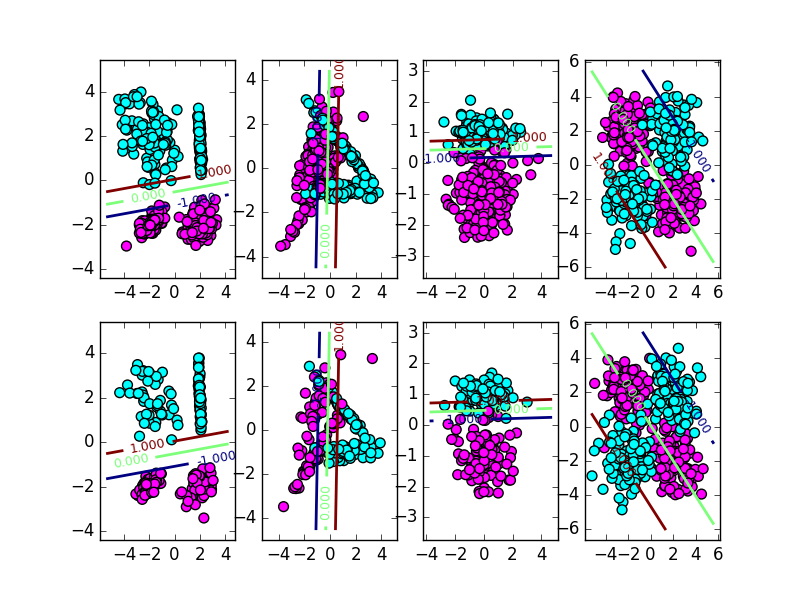
\includegraphics [trim=0 0 0 0, clip, angle=0, width=0.8\columnwidth,
	keepaspectratio]{figures/2_2_decisions}
	\caption{Four 2D datasets (positive elements in cyan, negative in magenta) are separated by SVM. The top row is the four training datasets, and the bottom row is the four corresponding validation sets.
	The three lines are the decision boundary ($\hat{y}=0.0$ in green) and positive and negative margin boundaries ($\hat{y}=\pm1.0$ in red/blue).}
	\label{fig:2_2_decisions} 
\end{figure}

\subsection{Part 3}
[todo]

